\documentclass[
  a4paper,
  12pt,
  spanish,
]{scrartcl}

% Párrafos
\setlength{\parindent}{18pt}
\linespread{1.05}

%-------------------------------------------------------------------------------
%	PAQUETES
%-------------------------------------------------------------------------------

% Idioma

\usepackage[es-noindentfirst, es-tabla]{babel}
\decimalpoint

% Citas de texto en línea/bloque

\usepackage[autostyle]{csquotes}

% Tablas

\usepackage{booktabs}
\usepackage{multirow}

% Matemáticas

\usepackage{amsmath, amsthm, amssymb}
\usepackage{mathtools}
\usepackage{commath}

% Fuentes personalizadas para utilizar con XeLaTeX o LuaLaTeX

\usepackage[no-math]{fontspec}
\setmainfont{Libertinus Serif}
\setsansfont{Libertinus Sans}
\setmonofont{Libertinus Mono}

\usepackage[math-style=TeX]{unicode-math}
\setmathfont{Libertinus Math}

% Configuración de microtype

\defaultfontfeatures{Ligatures=TeX,Numbers=Lining}
\usepackage[activate={true,nocompatibility},final,tracking=true,factor=1100,stretch=10,shrink=10]{microtype}
\SetTracking{encoding={*}, shape=sc}{0}

% Enlaces y colores

\usepackage{hyperref}
\usepackage[dvipsnames]{xcolor}
\definecolor{webgreen}{rgb}{0,0.5,0}
\hypersetup{
  colorlinks=true,
  citecolor=webgreen,
  urlcolor=Maroon,
  linkcolor=RoyalBlue
}

% Otros elementos de página

\usepackage{enumitem}
\setlist[enumerate]{leftmargin=*, itemsep=0pt}
\setlist[itemize]{leftmargin=*, itemsep=0pt}

\usepackage[labelfont=sc]{caption}
\usepackage[labelfont=default]{subcaption}
%\usepackage{graphicx}

% Tikz

\usepackage{tikz}
\usetikzlibrary{babel}
\usepackage{float}

% Código

\usepackage{listings}
\lstset{
	basicstyle=\footnotesize\ttfamily,%
	breaklines=true,%
	captionpos=b,                    % sets the caption-position to bottom
  tabsize=2,	                   % sets default tabsize to 2 spaces
  frame=lines,
  numbers=left,
  stepnumber=1,
  aboveskip=12pt,
  showstringspaces=false,
}
\renewcommand{\lstlistingname}{Listado}

% Algoritmos

\usepackage[linesnumbered, vlined]{algorithm2e}
\SetAlFnt{\sffamily}
\newcommand{\mykwfont}{\bfseries\sffamily}
\SetKwSty{mykwfont}

\SetKwInput{KwIn}{Entrada}%
\SetKwInput{KwOut}{Salida}%

\SetAlCapSkip{1em}
\SetAlCapFnt{\normalfont\scshape}

% Bibliografía

\usepackage[sorting=none, style=apa, isbn=true]{biblatex}
\DefineBibliographyStrings{spanish}{
  urlseen = {Consultado},
  retrieved = {Consultado},
}
\addbibresource{bibliografia.bib}

% Lorem ipsum

\usepackage{blindtext}

% Márgenes
\usepackage[bottom=3.125cm, top=2.5cm, left=4.5cm, right=4.5cm, marginparwidth=70pt]{geometry}

% Fuentes

\usepackage{textcase}

\newfontfamily{\sacshape}{Libertinus Serif}[
  WordSpace={1.8},
  LetterSpace={18.0}
]

\newfontfamily{\slscshape}{Libertinus Serif}[
  WordSpace={1.8},
  LetterSpace={6.0}
]

\DeclareRobustCommand{\spacedallcaps}[1]{{\linespread{1.3}\sacshape\MakeTextUppercase{#1}}}% WordSpace=1.8
\DeclareRobustCommand{\spacedlowsmallcaps}[1]{{\slscshape\MakeTextLowercase{#1}}}% WordSpace=1.8

% Cabeceras de sección

\RedeclareSectionCommands[beforeskip=-3ex,
afterskip=2ex]{section,subsection,subsubsection}
%\addtokomafont{section}{\normalfont\large\spacedallcaps}
%\setkomafont{section}{\normalfont\large\scshape}
\RedeclareSectionCommand[beforeskip=-9ex, font=\normalfont\large\scshape, tocentryformat=\normalfont\scshape]{section}
\addtokomafont{subsection}{\normalfont\normalsize\itshape}
\RedeclareSectionCommand[beforeskip=-6ex,tocentryformat=\normalfont\itshape]{subsection}
\addtokomafont{subsubsection}{\normalfont}
\RedeclareSectionCommand[beforeskip=-4ex]{subsubsection}
\addtokomafont{paragraph}{\normalfont\itshape}

% Entornos

\newtheoremstyle{teorema-style}  % Nombre del estilo
{1\topsep}                                  % Espacio por encima
{1\topsep}                                  % Espacio por debajo
{\itshape}                                  % Fuente del cuerpo
{0pt}                                  % Identación
{\scshape}                      % Fuente para la cabecera
{.}                                 % Puntuación tras la cabecera
{5pt plus 1pt minus 1pt}                              % Espacio tras la cabecera
{{\thmname{#1}\thmnumber{ #2}}\thmnote{ (#3)}}  % Especificación de la cabecera

\theoremstyle{teorema-style}
\newtheorem*{nth}{Teorema}

%-------------------------------------------------------------------------------
%	TÍTULO
%-------------------------------------------------------------------------------

\newcommand{\horrule}[1]{\rule{\linewidth}{#1}}

%-------------------------------------------------------------------------------
%	CONTENIDO
%-------------------------------------------------------------------------------

\begin{document}

\begin{titlepage}
  \vspace*{4cm}

  \begin{flushleft}
    \Huge
    \spacedallcaps{Redes neuronales artificiales}
    \horrule{2pt}
  \end{flushleft}

  \vspace{2em}

  \begin{flushright}
    \large
    Johanna Capote Robayna\\
    Antonio Coín Castro\\
    Guillermo Galindo Ortuño\\
    José María Martín Luque\\
    Luis Antonio Ortega Andrés\\
    Cristina de la Torre Villaverde
    \vspace{1em}

    \textit{Estadística Multivariante}

    Grado en Matemáticas

    \textsc{Universidad de Granada}\vspace{1em}

    \today\vspace{.5em}
  \end{flushright}
\end{titlepage}

\newpage

{\hypersetup{hidelinks}
\tableofcontents
}

\newpage

\section{Introducción}

El objetivo de este trabajo es el estudio del funcionamiento y de los fundamentos estadísticos de las redes neuronales artificiales.
Para ello indagaremos primeramente en el motivo de que se llamen así y las similitudes con las redes neuronales biológicas. Comenzaremos en la Sección \ref{sec:estructura} haciendo un recorrido histórico desde los inicios de las redes neuronales artificiales y comentando cómo ha ido evolucionando la estructura de las mismas, así como su proceso básico de funcionalmiento. En la Sección \ref{sec:teorema} justificaremos el nombre de \textit{aproximadores universales} con el que son referidas a veces las redes neuronales. Continuaremos en la Sección \ref{sec:diseño} explicando una serie de consideraciones a tener en cuenta a la hora de diseñar redes neuronales. En la Sección \ref{sec:clasificacion} realizaremos una clasificación (no exhaustiva) de las redes neuronales más populares en cuanto a diversos aspectos. Finalmente concluiremos en la Sección \ref{sec:ejemplos} presentando un par de ejemplos prácticos de aplicación de redes neuronales a un problema real, mostrando los resultados obtenidos.

Las cuestiones sobre la mente y el pensamiento humanos han estado presentes en el pensamiento filosófico desde sus inicios.
Posteriormente, el funcionamiento del cerebro y de la percepción humana han sido asuntos por los que la ciencia se ha interesado.
Actualmente es un campo interdisciplinario, la ciencia cognitiva, el que se encarga del estudio científico de la mente y sus procesos.
En concreto, se centra en la forma en la que el sistema nervioso procesa la información y cómo se produce el aprendizaje.
Trata además de responder diversas cuestiones sobre la mente y la inteligencia.
Para ello la ciencia cognitiva se sirve del conocimiento aportado por numerosos campos: psicología, antropología, neurociencia, filosofía, entre otros.

Uno de los modelos sobre cómo funcionan la mente y el cerebro es el conexionismo, cuyo principio básico es que los fenómenos mentales pueden describirse mediante redes compuestas por unidades sencillas (neuronas) e interconectadas entre sí.
En este modelo se han basado las redes neuronales artificales desde las primeras propuestas en la década de 1940.
Inicialmente las redes neuronales se diseñaron con el fin último de imitar la actividad cerebral.
Ahora se utilizan de forma más abstracta como una red de elementos de computación no lineales hiperconectados.

\begin{figure}[h]
  \centering
  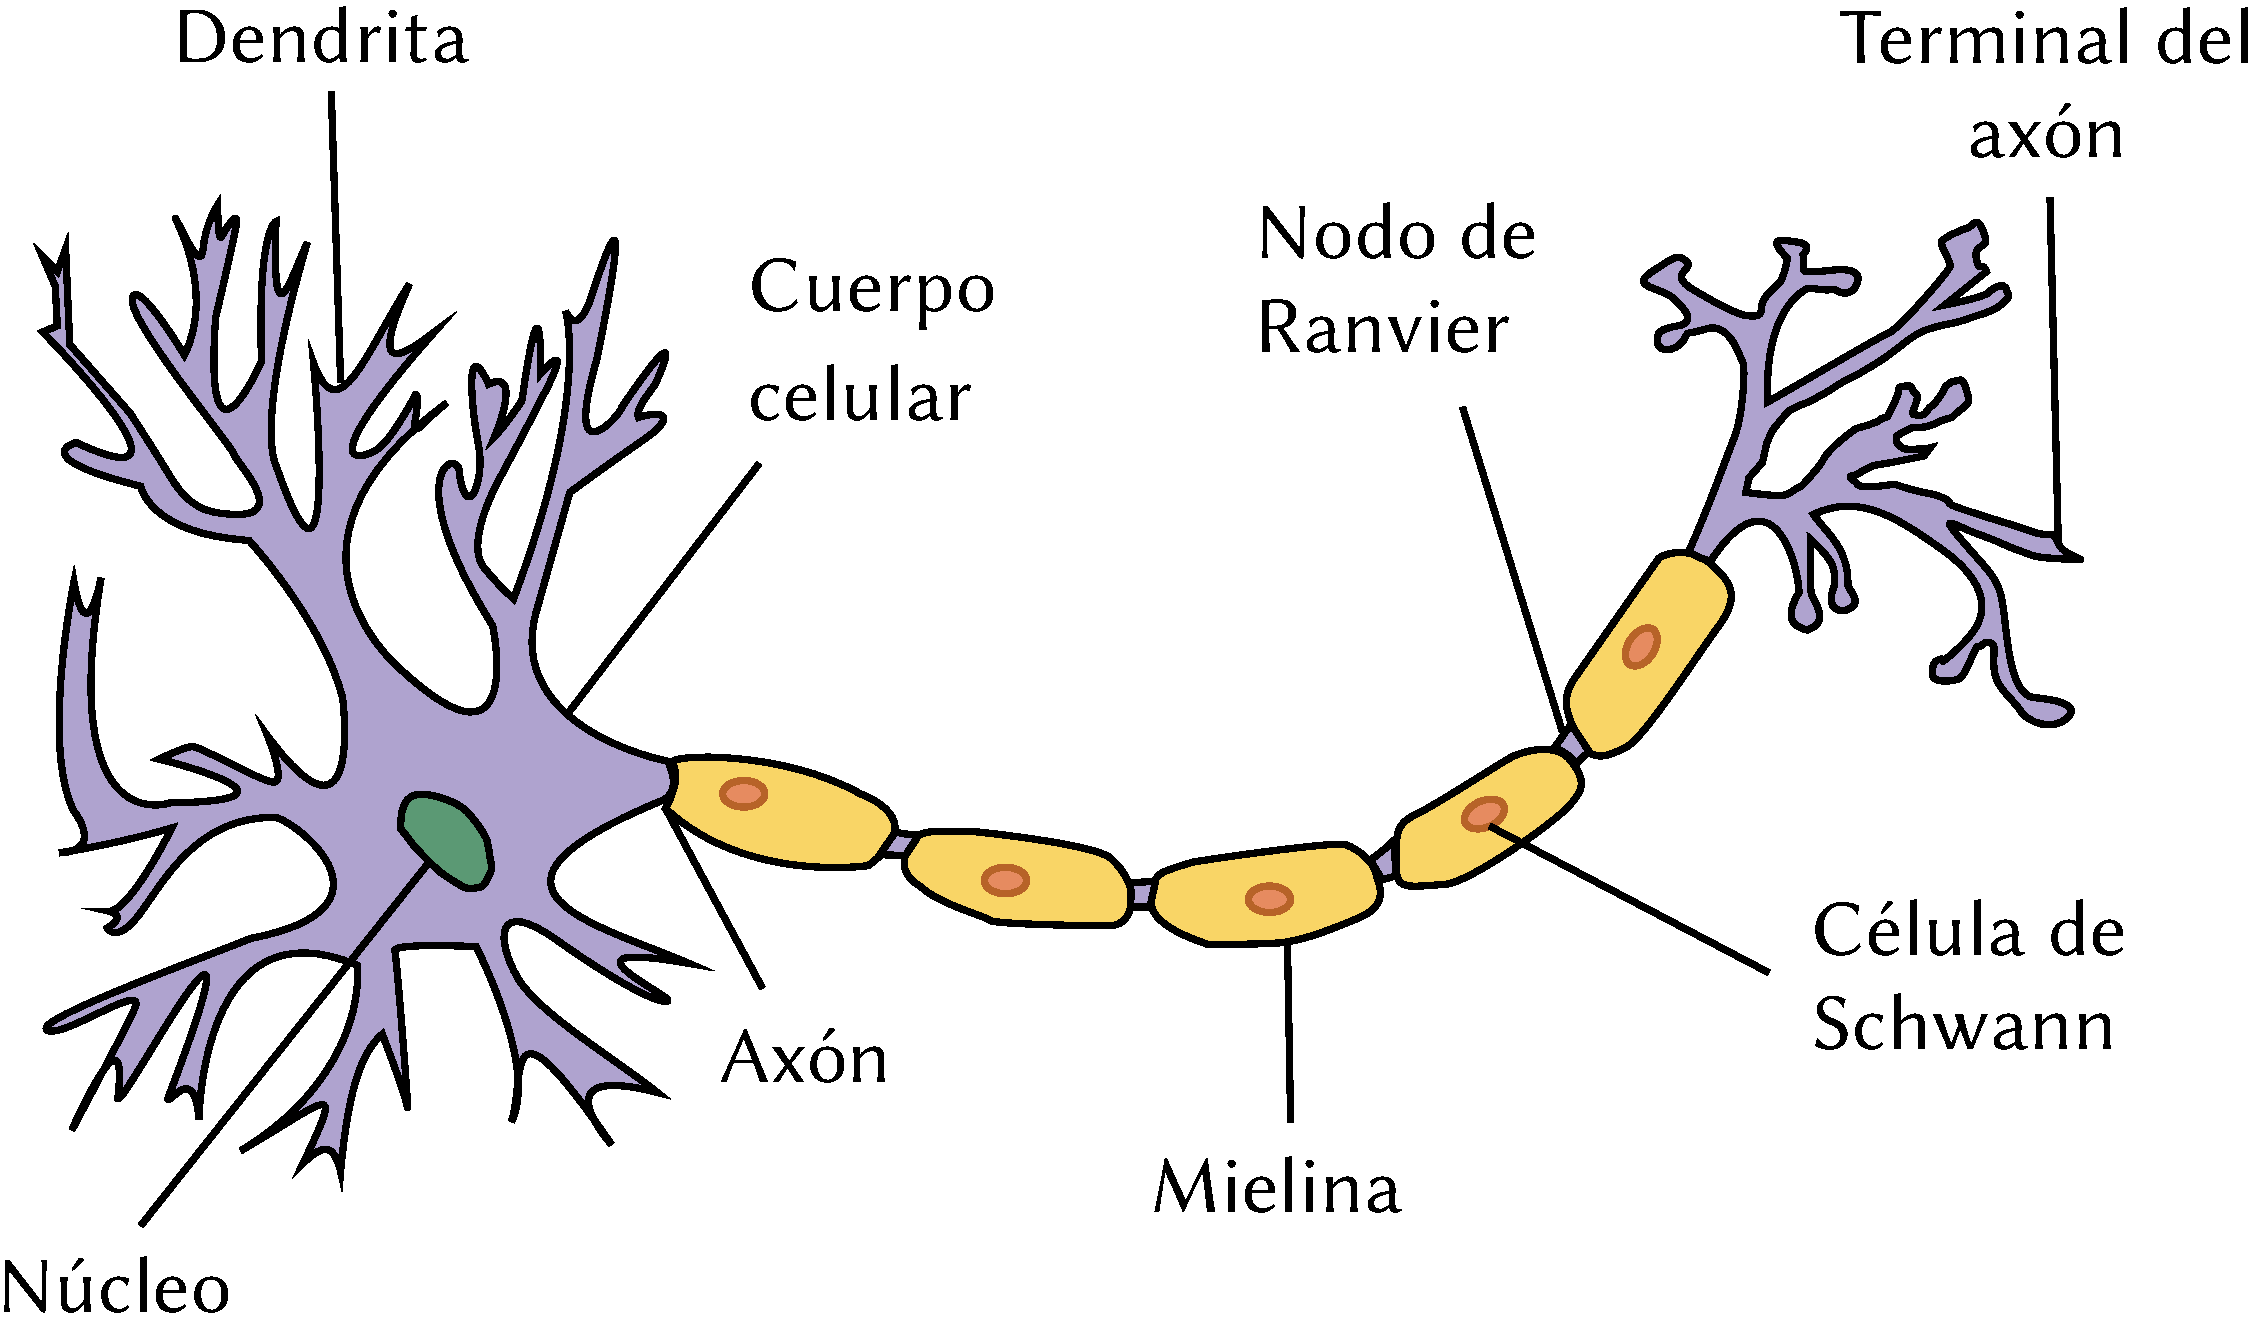
\includegraphics[width=0.7\textwidth]{img/neurona}
  \caption{Estructura de una neurona. Basada en \parencite{dhp1080_neurona_2007}.}
  \label{fig:neurona}
\end{figure}

Para entender cómo funciona una red neuronal artificial es útil comprender primero cómo funcionan las redes neuronales biológicas.
La corteza cerebral está formada por neuronas, células que son las unidades básicas que componen el sistema nervioso.
Los humanos poseen aproximadamente diez mil millones de neuronas.
En la estructura de una neurona, que podemos observar en la Figura \ref{fig:neurona}, es posible distinguir dos partes diferenciadas: el cuerpo celular y el axón.
En el cuerpo celular se encuentran las dendritas, que actúan como receptores de <<entrada>> de señales a la neurona.
El axón tiene forma alargada y actúa como emisor de <<salida>> de señales de la neurona.

Las neuronas se envían señales entre sí mediante un proceso electroquímico denominado sinapsis en el que se transmiten unas sustancias denominadas neurotransmisores.
El cerebro <<aprende>> cambiando la intensidad de las conexiones entre neuronas o creando o destruyendo dichas conexiones.
En el proceso de comunicación entre dos neuronas distinguimos entre la neurona \textit{presináptica}, la emisora, y la neurona \textit{postsináptica}, la receptora.
Para el envío de una señal la neurona presináptica envía neurotransmisores a través del axón a un conjunto de moléculas receptoras en la neurona postsináptica.
Este envío suele ocurrir en periodos de tiempo de duración aleatoria, pero la tasa de envío depende de muchos factores, entre ellos la intensidad de la señal de <<entrada>> a la neurona presináptica.
Esta intensidad se deriva de la proporción de dos tipos de sinapsis que recibe la neurona: las sinapsis inhibidoras, que previenen que la neurona envíe información, y las sinapsis excitadoras, que lo facilitan.

Veremos a continuación que los procesos diseñados para las redes neuronales artificales siguen un esquema prácticamente idéntico al que acabamos de describir.

\section{Estructura y funcionamiento de las redes neuronales}
\label{sec:estructura}

\subsection{La neurona de McCulloch-Pitts}

La neurona de McCulloch-Pitts \parencite{mcculloch_logical_1943} es un modelo computacional que consta de múltiples entradas a una unidad de procesamiento (imitando las dendritas) y una sola salida (imitando el axón). Las entradas se denotan por $X_1,X_2,\dots, X_r$ y la salida por $Y$, donde cada una puede tomar el valor $0$ (apagado) o $1$ (activado). Cada conexión puede ser de tipo excitador o inhibidor, y si alguna de ellas es inhibidora y transmite el valor $1$, la salida es directamente $0$. Si no hay conexiones inhibidoras activadas se suman las entradas para producir un valor de \textit{excitación total} $U = \sum_{j} X_j$, y se compara con un valor de \textit{umbral} $\theta$: si $U \ge \theta$ la salida es $Y=1$, en otro caso la salida es $Y=0$. Notamos que si $\theta > r$ la salida siempre será $0$, y si $\theta = 0$ y no hay conexiones inhibidoras activadas, la salida será siempre $1$. Podemos ver una ilustración de esta neurona en la Figura \ref{fig:mcculloch-pitts}.

\begin{figure}[h]
  \centering
  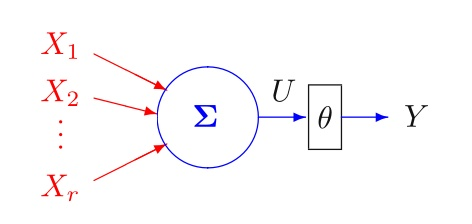
\includegraphics[width=.7\textwidth]{img/mcculloch-pitts}
  \caption{Neurona de McCulloch-Pitts con $r$ entradas binarias $X_1,\dots,X_r$, una salida binaria $Y$ y un umbral $\theta$. Extraída de \parencite{izenman_modern_2008}.}
  \label{fig:mcculloch-pitts}
\end{figure}

Observamos que para un valor fijo de $\theta$, la neurona de McCulloch-Pitts divide el espacio de entrada en dos mitades determinadas por el hiperplano $\sum_j X_j = \theta$; los puntos $(X_1, \dots, X_r)$ con salida $Y=1$ quedan a un lado del hiperplano, mientras que aquellos con $Y=0$ quedan en el otro lado.

A modo de ejemplo, podemos utilizar esta neurona para implementar las funciones lógicas AND y OR de $r$ entradas. Para la función AND elegimos como umbral $\theta = r$, y así la salida tomará el valor 1 únicamente cuando todas las entradas sean 1. Para la función OR elegimos como umbral $\theta = 1$ para que la salida sea $1$ en cuanto alguna de las entradas sea $1$. La construcción de la función NOT es también inmediata, sin más que considerar una única entrada inhibidora y un umbral de $0$, por lo que combinando neuronas de McCulloch-Pitts podemos construir cualquier función booleana.

A pesar de la universalidad mostrada, este modelo no es adecuado para realizar un proceso de aprendizaje, pues la única forma de resolver diferentes problemas es ir cambiando el número y tipo de las entradas y el valor del umbral. Esto hizo que se perdiese rápidamente el interés en este modelo computacional.

\subsection{Perceptrón de una capa}

A principios de los años 60 se produjo una segunda oleada de interés en las redes neuronales artificales, cuando el psicólogo Frank Rosenblatt desarrolló un sistema llamado \textit{perceptrón} \parencite{rosenblatt_perceptron_1958} para imitar el funcionamiento de una neurona. Se trata básicamente de una neurona de McCulloch-Pitts dotada de unos \textit{pesos} $\beta_i \in \mathbb{R}$ en cada conexión $i=1,2,\dots, r$. Los pesos positivos representan conexiones excitadoras, los pesos negativos conexiones inhibidoras y la magnitud de los mismos muestra la fuerza de la conexión.

En este caso, se calcula la suma ponderada $U=\sum_j \beta_j X_j$, y la neurona se activa únicamente si $U\ge \theta$. Podemos convertir el umbral a $0$ introduciendo un elemento de \textit{sesgo} $\beta_0 = -\theta$ y una nueva pseudovariable $X_0 = 1$. De esta forma, como $U-\theta = \beta_0 + U$, podemos simplemente comparar $U=\sum_{j=0}^r \beta_j X_j$ con $0$. En la Figura \ref{fig:perceptron} podemos ver un esquema de un perceptrón descrito de esta forma.

\begin{figure}[h]
  \centering
  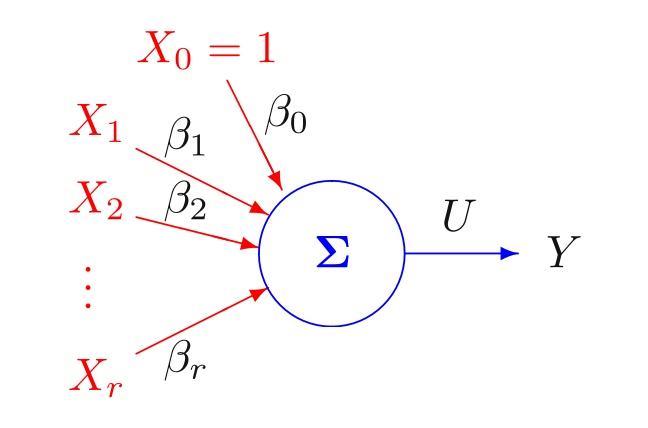
\includegraphics[width=.7\textwidth]{img/perceptron}
  \caption{Perceptrón de $r$ entradas binarias con pesos $\{\beta_j\}$ y salida binaria $Y$. Incluye el término de sesgo $\beta_0$. Extraída de \parencite{izenman_modern_2008}.}
  \label{fig:perceptron}
\end{figure}

Si los datos de entrada son \textit{linealmente separables} (es decir, se pueden separar por un hiperplano), podemos interpretar un perceptrón como un algoritmo de \textit{clasificación binaria}, de forma que los puntos con $Y=0$ pertenecen a una clase distinta a la de aquellos con $Y=1$; la partición queda determinada por el hiperplano $U=\theta$. Sin embargo, si los datos de entradan no son linealmente separables, la función $Y$ asociada no es computable por un perceptrón (un ejemplo de este caso es la función XOR). En la Figura \ref{fig:separable} puede verse una representación gráfica de datos separables y no separables linealmente.

\begin{figure}[h]
  \centering
  \begin{subfigure}[b]{0.4\textwidth}
    \centering
    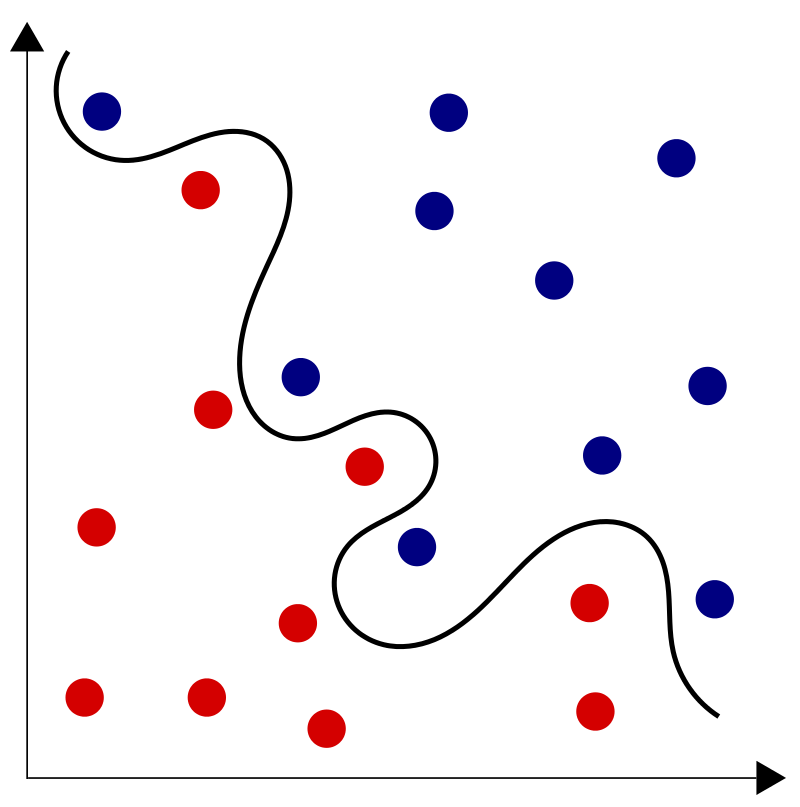
\includegraphics[width=.8\textwidth]{img/non-separable}
    \caption{No linealmente separables}
  \end{subfigure}
  \qquad
  \begin{subfigure}[b]{0.4\textwidth}
    \centering
    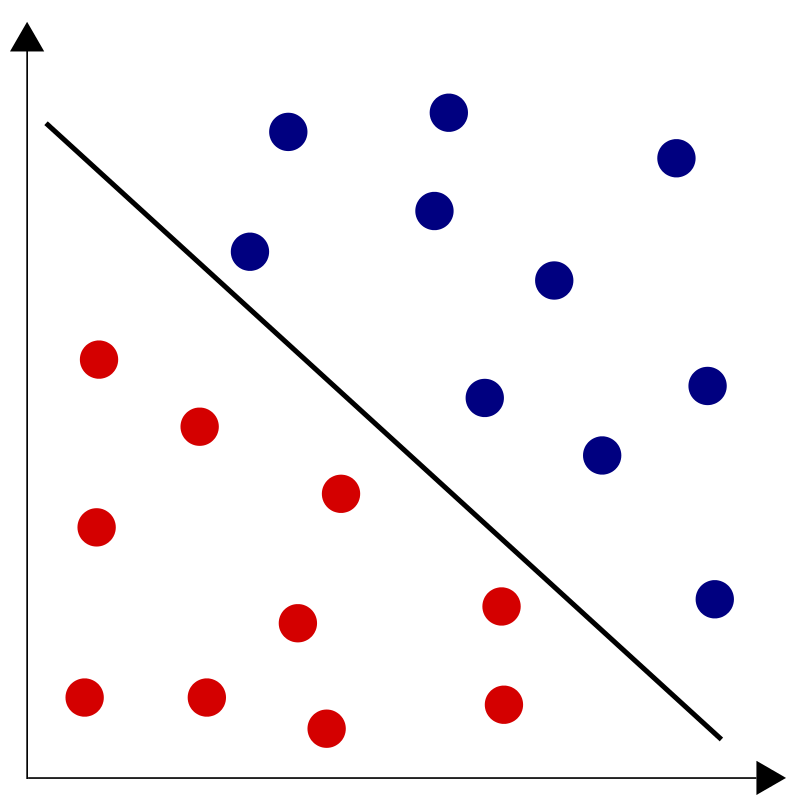
\includegraphics[width=.8\textwidth]{img/separable}
    \caption{Linealmente separables}
  \end{subfigure}
  \caption{Ejemplos de datos bidimensionales separables y no separables linealmente. Extraída de \parencite{wikipedia_separable}.}
  \label{fig:separable}
\end{figure}

Podemos considerar una red neuronal de perceptrones interconectados organizados en dos grupos: $r$ nodos de entrada $\{X_j\}$ y $s$ nodos de salida $\{Y_k\}$, que pueden tomar tanto valores reales como discretos. Cada conexión $X_j \to Y_k$ está marcada por un peso $\beta_{jk}$. Este tipo de redes se conocen como \textit{redes de una capa}, pues aunque hay dos grupos solo se realizan cálculos significativos en los nodos de salida.

\subsection{Funciones de activación}

El objetivo ahora es construir una red de una capa que dado un problema sea capaz de aprender unos pesos para resolverlo. No es difícil darse cuenta de que hasta ahora en cada perceptrón solo hemos computado una transformación afín de los datos de entrada: si $\mathbf{X}=(X_1, \dots, X_r)^T$ es un vector aleatorio de entradas y tenemos $s$ nodos de salida, en cada uno de ellos calculamos
\[
U_k = \beta_{0k} + \mathbf{X}^T \pmb\beta_k, \quad k = 1,\dots, s,
\]
donde $\beta_{0k}$ es la constante de \textit{sesgo} y $\pmb{\beta}_k = (\beta_{1k}, \dots, \beta_{rk})^T$ es un vector de pesos. De esta forma la red no podría aprender funciones que tengan un comportamiento no lineal, y es por esto que se introduce el concepto de \textit{función de activación}. Consideramos una función no lineal $f$ que se aplica a la salida de cada nodo, de forma que la salida final obtenida es
\[
U_k = f(\beta_{0k} + \mathbf{X}^T \pmb{\beta}_k), \quad k = 1,\dots, s.
\]

Ejemplos de funciones de activación comunes son \textit{sigmoides} como la función logística o la tangente hiperbólica, y también la función \textit{signo} para problemas de clasificación binaria. En los últimos años se ha popularizado el uso de la función ReLU dada por $f(x) = x^+ = \max{\{0, x\}}$, cuya gráfica podemos ver en la Figura \ref{fig:relu}.

\begin{figure}[h]
  \centering
  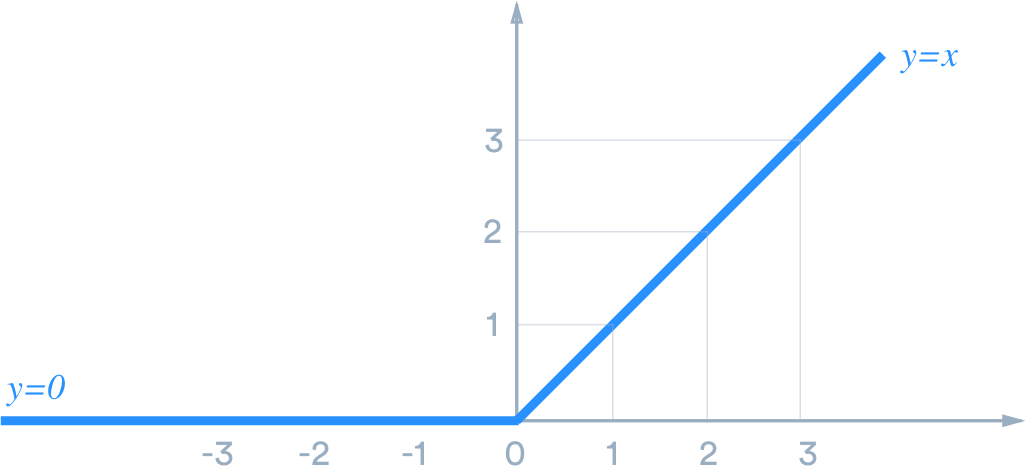
\includegraphics[width=.7\textwidth]{img/relu}
  \caption{Gráfica de la función ReLU.}
  \label{fig:relu}
\end{figure}

En el contexto de problemas de \textit{clasificación multiclase} podemos considerar también una función de activación vectorial $\pmb f$ aplicada al vector de \textit{outputs} $\pmb U = (U_1, \dots, U_s)^T$. Por ejemplo, la función \textit{softmax} $\pmb f(\pmb x)_i = e^{x_i}/\sum_{k=1}^s e^{x_k}$ se puede entender como una distribución de probabilidad en $s$ valores, de forma que la salida en el nodo $k$-ésimo representa la probabilidad de pertenecer a la $k$-ésima clase.

\subsection{Proceso de aprendizaje}

La clave del funcionamiento de esta arquitectura es que se puede definir un proceso iterativo mediante el cual la red es capaz de \textit{aprender} los pesos óptimos para resolver un problema de clasificación binaria. Suponemos que tenemos una serie de ejemplos de entrada independientes $\pmb X_1, \dots, \pmb X_n$ extraídos de dos clases $\Pi_1$ y $\Pi_2$, y un único nodo de salida. Incorporando el valor del sesgo al vector de pesos y adoptando la notación $\pmb \beta \leftarrow (\beta_0, \pmb \beta^T)^T$ y $\pmb X \leftarrow (1, \pmb X^T)^T$, podemos reescribir $\beta_{0} + \mathbf{X}^T \pmb{\beta}$ como $\mathbf{X}^T \pmb{\beta}$. Para un estado concreto de la red (es decir, unos pesos fijos $\pmb \beta$), interpretaremos que un ejemplo $\pmb X$ pertenece a la primera clase si y solo si $\pmb X^T \pmb \beta \ge 0$. La estrategia es utilizar el conocimiento de la clase correcta para ir pasando los ejemplos por la red y predecir la clase a la que pertenece cada uno, intentando corregir los pesos si se detecta un error. Esta técnica se conoce como \textit{aprendizaje supervisado}.

La regla para actualizar los pesos en cada iteración es la siguiente:
\begin{enumerate}
  \item Si la versión actual de los pesos $\pmb \beta_h$ consigue clasificar correctamente $\pmb X_h$, no cambiamos los pesos para la siguiente iteración.
  \item Si con los pesos $\pmb \beta_h$ no obtenemos una clasificación correcta, hacemos
\[
  \pmb \beta_{h+1} = \pmb \beta_h + \eta \operatorname{signo}(\pmb X^T_h \pmb \beta_h) \pmb X_h.
\]
El parámetro $\eta > 0$ se conoce como \textit{learning rate}, y controla en qué proporción varían los pesos en cada iteración.
\end{enumerate}

Una solución del problema será un vector de pesos $\pmb \beta^\ast$ que clasifique correctamente todos los ejemplos, es decir, que todos los que estén a un mismo lado de cada hiperplano $\pmb X_h^T \pmb \beta^\ast$ pertenezcan a la misma clase. Para esto es necesario que los datos de entrada sean linealmente separables. La utilización de este método se justifica gracias al siguiente resultado.

\begin{nth}[Convergencia del perceptrón]
Para un problema de clasificación binaria con clases linealmente separables, si existe una solución $\pmb \beta^\ast$, el algoritmo descrito anteriormente la encontrará en un número finito de iteraciones.
\end{nth}

Este algoritmo se puede extender a problemas de clasificación multiclase. Dada una \textit{función de error} diferenciable $F(\pmb x)$ que mida la diferencia entre la clase predicha y la clase real, se utiliza un algoritmo de \textit{gradiente descendente} que propaga hacia atrás el error en cada iteración y modifica los pesos de acuerdo a la regla
\[
\pmb \beta_{h+1} = \pmb \beta_h - \eta \nabla F_h(\pmb \beta_h).
\]
Notamos que perseguimos minimizar la función de error avanzando en la dirección y sentido de máxima pendiente: la que marca el gradiente cambiado de signo.

\subsection{Perceptrón multicapa}

A mediados de los años 80 se acuñó finalmente el concepto de \textit{perceptrón multicapa}. Se trata de un modelo que pretende solventar las limitaciones del perceptrón distribuyendo los nodos en varias capas y aplicando transformaciones no lineales en el paso de una capa a la siguiente. Las capas intermedias se conocen como \textit{capas ocultas}. Podemos ver un esquema de este modelo en la Figura \ref{fig:multi}.

\begin{figure}[h]
  \centering
  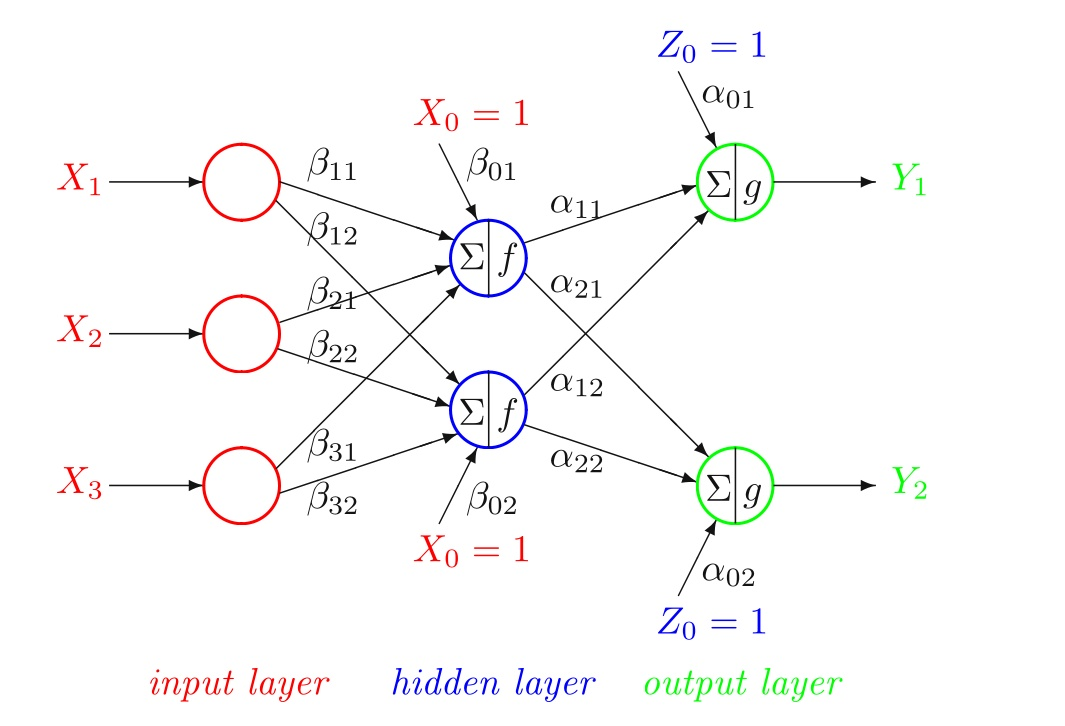
\includegraphics[width=.8\textwidth]{img/multicapa}
  \caption{Esquema de un perceptrón multicapa totalmente conectado con una capa oculta. Extraída de \parencite{izenman_modern_2008}.}
  \label{fig:multi}
\end{figure}

En general, una red con $L$ capas ocultas se conoce como una red de $L+1$ capas (de nuevo, la capa de entrada no cuenta). Decimos que una capa está \textit{totalmente conectada} cuando todos sus nodos reciben como entrada activaciones de todas las neuronas de la capa anterior, y \textit{parcialmente conectada} en otro caso. Recientemente se empezó a utilizar el concepto de \textit{redes profundas} ó \textit{deep neural networks} para referirse a redes con varias capas ocultas.

Para el proceso de aprendizaje de la red, se utiliza de nuevo la técnica de gradiente descendente, pero esta vez se va propagando hacia atrás el error en todas las capas, alterando todos los pesos en el proceso de forma iterativa.

Una vez que tenemos unos pesos \textit{suficientemente buenos}, podemos utilizar la red entrenada para clasificar nuevos ejemplos no etiquetados que no ha visto antes, aspirando así a resolver el problema de clasificación en todo el espacio de entrada. La bondad o \textit{precisión} de la red se medirá, dado un conjunto de \textit{test} con nuevos ejemplos, contando el número de de ellos que ha sido capaz de clasificar correctamente.

También podemos abordar el problema de regresión lineal múltiple mediante redes neuronales. En particular, si consideramos una red con un único nodo de salida y que utilice únicamente funciones de activación lineal, podremos entrenarla para que aprenda los pesos (coeficientes) de la función lineal que mejor aproxima los datos de entrada. Si utilizamos como función de error el error cuadrático, estaríamos ante una regresión por mínimos cuadrados.

Del mismo modo se puede entender una red con activaciones no lineales como una manera de realizar una regresión no lineal a partir de los datos de entrenamiento. Si estos últimos no tienen ruido, nos encontraríamos ante un problema de aproximación de funciones.

Podemos preguntarnos cómo se comparan las redes neuronales en términos de rendimiento con las técnicas estadísticas clásicas que pretenden resolver los mismos problemas. Un punto en contra de los modelos basados en redes neuronales es que sufren de \textit{pérdida de interpretabilidad} frente a modelos clásicos. A cambio, las redes neuronales consiguen resolver problemas mucho más complejos de forma automática, en parte gracias a la gran capacidad de cómputo de la que disponen los ordenadores hoy en día. Sin embargo, debemos tener en cuenta que el tiempo de entrenamiento de una red neuronal para resolver un problema complejo puede ser muy elevado, y depende de varios factores como el tamaño del conjunto de entrenamiento, la anchura y profundidad de la red o el número de conexiones entre neuronas.

\section{El teorema de aproximación universal}
\label{sec:teorema}

En la teoría matemática de las redes neuronales artificiales, un teorema muy celebrado es el \textit{teorema de aproximación universal} demostrado inicialmente por George Cybenko en 1989. Este teorema establece que una red \textit{feed-forward} con una sola capa oculta que contiene un número finito de neuronas puede aproximar con precisión arbitraria cualquier función continua en un subconjunto compacto de $\mathbb{R}^n$, bajo condiciones poco restrictivas sobre la función de activación.

El teorema da cuenta de la gran expresividad que poseen las redes neuronales, pues dice que, si las funciones de activación son no polinómicas, las redes neuronales simples pueden representar una amplia variedad de funciones interesantes cuando se les proporcionan parámetros apropiados. Sin embargo, no dice nada sobre la capacidad de aprendizaje algorítmico de esos parámetros.

Aunque las redes \textit{feed-forward} con una sola capa oculta son aproximadores universales, el ancho de tales redes crece de forma exponencial. En el año 2017 los investigadores Zhou Lu, Hongming Pu, Feicheng Wang y otros \parencite{lu_expressive_2017} probaron el teorema de aproximación universal para redes neuronales profundas con ancho acotado. En particular, demostraron que las redes de ancho $n + 4$ con funciones de activación ReLU pueden aproximar cualquier función Lebesgue-integrable en el espacio de entrada $n$-dimensional con respecto a la distancia $L^{1}$ si la profundidad de la red puede crecer.

Matemáticamente la expresión del teorema se puede expresar en dos versiones, la aplicada a un ancho no acotado y a un ancho acotado, que vamos a comentar a continuación.

\subsection{Caso ancho no acotado}

Sea $\varphi:\mathbb{R} \rightarrow \mathbb{R}$ una función no constante, acotada y continua, llamada \textit{función de activación} y sea $I_m$ el hipercubo unidad de dimensión $m$, $[0,1]^m$.
Entonces, dado un valor $\varepsilon > 0$ y una función $f \in C(I_m)$, existen un valor entero $N$, unas constantes $v_i , b_i \in \mathbb{R}$ y unos vectores de pesos $\pmb{w}_i \in \mathbb{R}^m$, para $i =1 \cdots N$, tales que podemos definir la función
\[
  F (x) = \sum_{{i = 1}}^{{N}} v_{i} \varphi \left (\pmb w_ {i} ^ {T} x + b_ {i} \right)
\]
como una realización aproximada de la función $f$, es decir, se verifica que
\[
  |F(x)-f(x)| < \varepsilon
\]
para todo \(x \in I_m\).
En otras palabras, las funciones de la forma $F(x)$ son densas en $C(I_m)$.
Esto es válido también si tomamos cualquier subconjunto compacto de $\mathbb{R}^m$ en lugar de $I_m$.

\subsection{Caso ancho acotado}

Para cualquier función Lebesgue-integrable $f: \mathbb{R}^n \rightarrow \mathbb{R}$ y cualquier $\varepsilon >0$, existe una red completamente conectada con activación ReLU \(\mathcal A\) con ancho menor que $n+4$, tal que la función $F_{\mathcal A}$ representada por esta red verifica que
\[
  \displaystyle \int_{\mathbb{R}^{n}}\left|f(x)-F_{\mathcal A}(x)\right|\dif x < \varepsilon.
\]

\section{Consideraciones de diseño en redes neuronales}
\label{sec:diseño}

A la hora de diseñar una red neuronal para resolver un problema debemos tener en cuenta las particularidades de los datos a los que nos enfrentamos, así como la información de la que disponemos sobre el problema. Es decir, para obtener unos buenos resultados es necesario realizar un análisis previo de la situación que nos permita optimizar el diseño de la red y ajustarlo al problema concreto con el que tratamos. A continuación enumeramos las principales consideraciones a tener en cuenta.

\subsection{Capacidad de generalización}

Uno de los mayores problemas que ocurren durante el entrenamiento de una red neuronal se denomina \textit{overfitting} o sobreajuste. Este fenómeno se produce cuando el error en el conjunto de entrenamiento alcanza un valor muy pequeño porque los datos se han ajustado demasiado a unos pocos ejemplos concretos, llegando incluso a <<memorizarlos>>. Esto provocará que al presentar nuevos ejemplos a la red, esta no sea capaz de generalizar lo aprendido y los clasifique de forma errónea. En la Figura \ref{fig:overfitting} podemos ver una representación gráfica de este hecho, viendo cómo la precisión en el conjunto de entrenamiento aumenta indefinidamente mientras que la precisión en el conjunto de validación comienza a caer.

\begin{figure}[h]
  \centering
  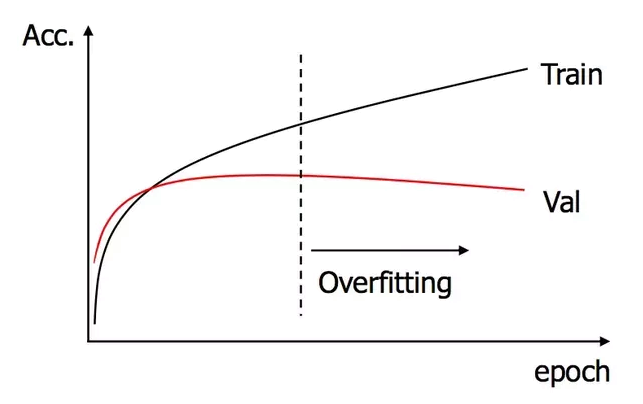
\includegraphics[width=.7\textwidth]{img/overfitting}
  \caption{Gráficas de precisión en el conjunto de entrenamiento y de validación cuando se produce sobreajuste.}
  \label{fig:overfitting}
\end{figure}

Para evitar este problema es posible aplicar técnicas de \textit{regularización} durante el entrenamiento que obliguen a la red a no ajustarse demasiado a los datos de entrenamiento. Un ejemplo de esto sería apagar de forma aleatoria algunas neuronas durante el entrenamiento.

\subsection{Caída en óptimos locales}

Una situación muy común en el contexto de las redes neuronales es que tras un período de entrenamiento se alcance un mínimo local de la función de error, y la red ya no consiga seguir aprendiendo para disminuirlo aún más el error. Para controlar este fenómeno se ajusta el parámetro de \textit{learning rate} o tasa de aprendizaje. Como ya comentamos, este parámetro es el que indica cuánto hay que cambiar los pesos del modelo en respuesta al error estimado cada vez que se realiza un pase hacia delante de los datos por la red.

Elegir el valor apropiado de \textit{learning rate} puede ser una tarea muy complicada, ya que un valor demasiado pequeño puede acarrear que el error de que la red no se optmice en el proceso de entrenamiento, mientras que elegir un parámetro demasiado elevado puede llevar a la que red caiga en óptimos locales y deje de aprender. Podemos ver un estudio del comportamiento de la red en función de este parámetro en la Figura \ref{fig:learning-rate}.

\begin{figure}[h]
  \centering
  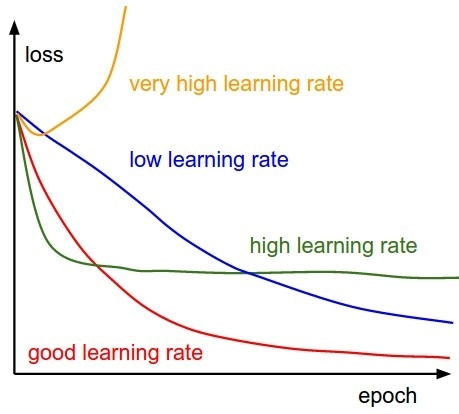
\includegraphics[width=.65\textwidth]{img/learning-rate}
  \caption{Evolución de la función de pérdida en función del \textit{learning rate} elegido.}
  \label{fig:learning-rate}
\end{figure}

\subsection{Transferencia de conocimiento}

Una idea clave que rodea a las redes neuronales de más de una capa es que se estratifica el procesamiento de los datos, y cada capa se encarga de <<aprender>> una serie de características que van de lo general a lo particular. Es por esto que podemos aprovechar una red ya entrenada con un número elevado de datos para aplicarla a un problema distinto.

Por ejemplo, si suponemos una red entrenada para un problema de clasificación en $K$ clases, podemos eliminando de la misma la últimas capa encargada de realizar la clasificación y sustituirla por otra capa de nuestra elección con $M \neq K$ clases. Podemos usar esta nueva red preentrenada para clasificar nuevos datos, siempre que estos tengan alguna relación con los datos con los que fue entrenada la red.

\section{Clasificación de redes neuronales}
\label{sec:clasificacion}

Las redes neuronales se pueden clasificar según el paradigma de entrenamiento que utilicen:

\begin{enumerate}
\item \textit{Aprendizaje supervisado. } Junto con el conjunto de datos de entrada entrada se proporciona un conjunto de etiquetas que representan la salida deseada. El trabajo de la red consiste en reproducir la salida deseada para cada entrada. Para conseguirlo trata de minimizar el error entre la salida de la red y la salida esperada. Este tipo de aprendizaje se suele utilizar en reconocimiento de patrones, clasificación y regresión.
\item \textit{Aprendizaje no supervisado. } En este tipo de entrenamiento, los
  datos de entrada se dan junto con una función de coste (una función de los
  datos y la salida de la red). El objetivo de la red es minimizar dicha función
  de coste. Estas redes se utilizan generalmente para resolver problemas de
  estimación y clustering.
\item \textit{Aprendizaje por refuerzo. } El objetivo de este tipo de
  entrenamiento es hacer que la red adapte una politica de acción que resulte en elegir la mejor acción posible en cada estado para maximizar una \textit{función de recompensa}. Se utiliza en problemas de optimización de control, y puede realizarse el entrenamiento en tiempo real.
\end{enumerate}

Presentamos ahora algunos tipos de redes atendiendo principalmente a su topología.

\subsection{Redes convolucionales}%
\label{sub:redes_convolucionales}

Las redes neuronales convolucionales son un tipo de red que han sido muy efectivas en áreas relacionadas con las imágenes, como el reconocimiento o clasificación de estas.

Una de las principales diferencias con las redes neuronales usuales es que la entrada de estas es una imagen con tres canales (R, G, B), por ejemplo, un tensor de tamaño $32\times 32 \times 3$, en lugar de un vector de entradas como en las redes neuronales tradicionales.

A continuación explicaremos el concepto de convolución, que es el principal motivo por el que este tipo de redes son tan útiles. Continuando con el ejemplo, supongamos que tenemos una imagen representada por un tensor de naturales de tamaño $32\times 32 \times 3$, y consideremos también otro tensor de menor tamaño, por ejemplo $5 \times 5 \times 3$, que será el \textit{filtro} o núcleo de la convolución. Entonces, aplicar la convolución del núcleo mencionado con la imagen consiste en <<desplazarlo>> por todas las posibles posiciones de la matriz, y aplicar el producto elemento a elemento entre la submatriz y el filtro. En la Figura \ref{fig:conv} mostramos un imagen que ejemplifica este proceso.

\begin{figure}[h]
    \centering
    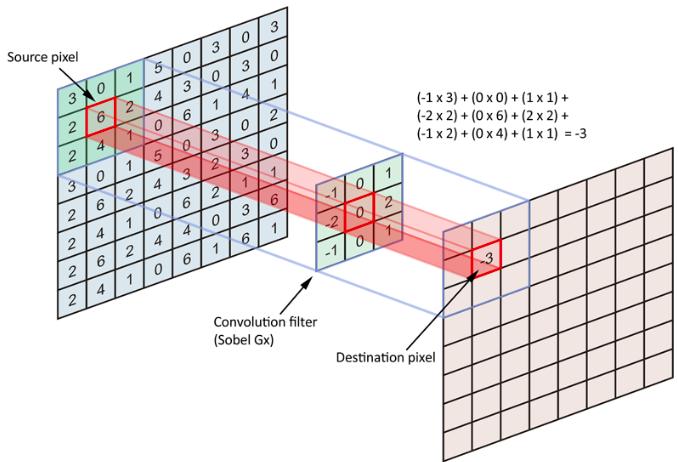
\includegraphics[width=0.7\linewidth]{img/conv.png}
    \caption{Ejemplo de convolución de una imagen. Extraído de \parencite{arden_cnn_2017}.}%
    \label{fig:conv}
\end{figure}

Dicho esto, una capa de una red convolucional consiste en una serie de filtros a aplicar a la imagen resultante de la capa anterior, siendo los valores de dichos filtros los pesos que queremos estimar.

En general, las primeras capas de una red convolucional son las encargadas de extraer las características más generales de la imagen, mientras que las más profundas utilizan la información extraída por las capas anteriores, capturando carácterísticas más específicas. Finalmente, se añade una capa completamente conectada, que es la encargada de realizar la clasificación de la imagen con las características recogidas.

Este tipo de redes son muy útiles gracias a la multitud de propiedades que tiene la operación de convolución (conmutatividad, asociatividad, distributividad, ...), y a que sería inviable entrenar una red completamente conectada que trabajase con imágenes de tamaño elevado, pues el número de parámetros sería demasiado grande.

\subsection{Autoencoders}

Un \textit{autoencoder} es un tipo de red neuronal de aprendizaje no supervisado que aprende a copiar su entrada en la
salida. Tiene una capa interna que constituye el <<código>> con
el que queremos representar la entrada, y se encuentra dividida en dos partes principales:
\begin{enumerate}
  \item \textit{Codificador. } Conjunto de capas que transforman la entrada al <<código>>.
  \item \textit{Decodificador. } Conjunto de capas que transforman el <<código>> a la entrada original.
\end{itemize}

\begin{figure}[h]
  \centering
  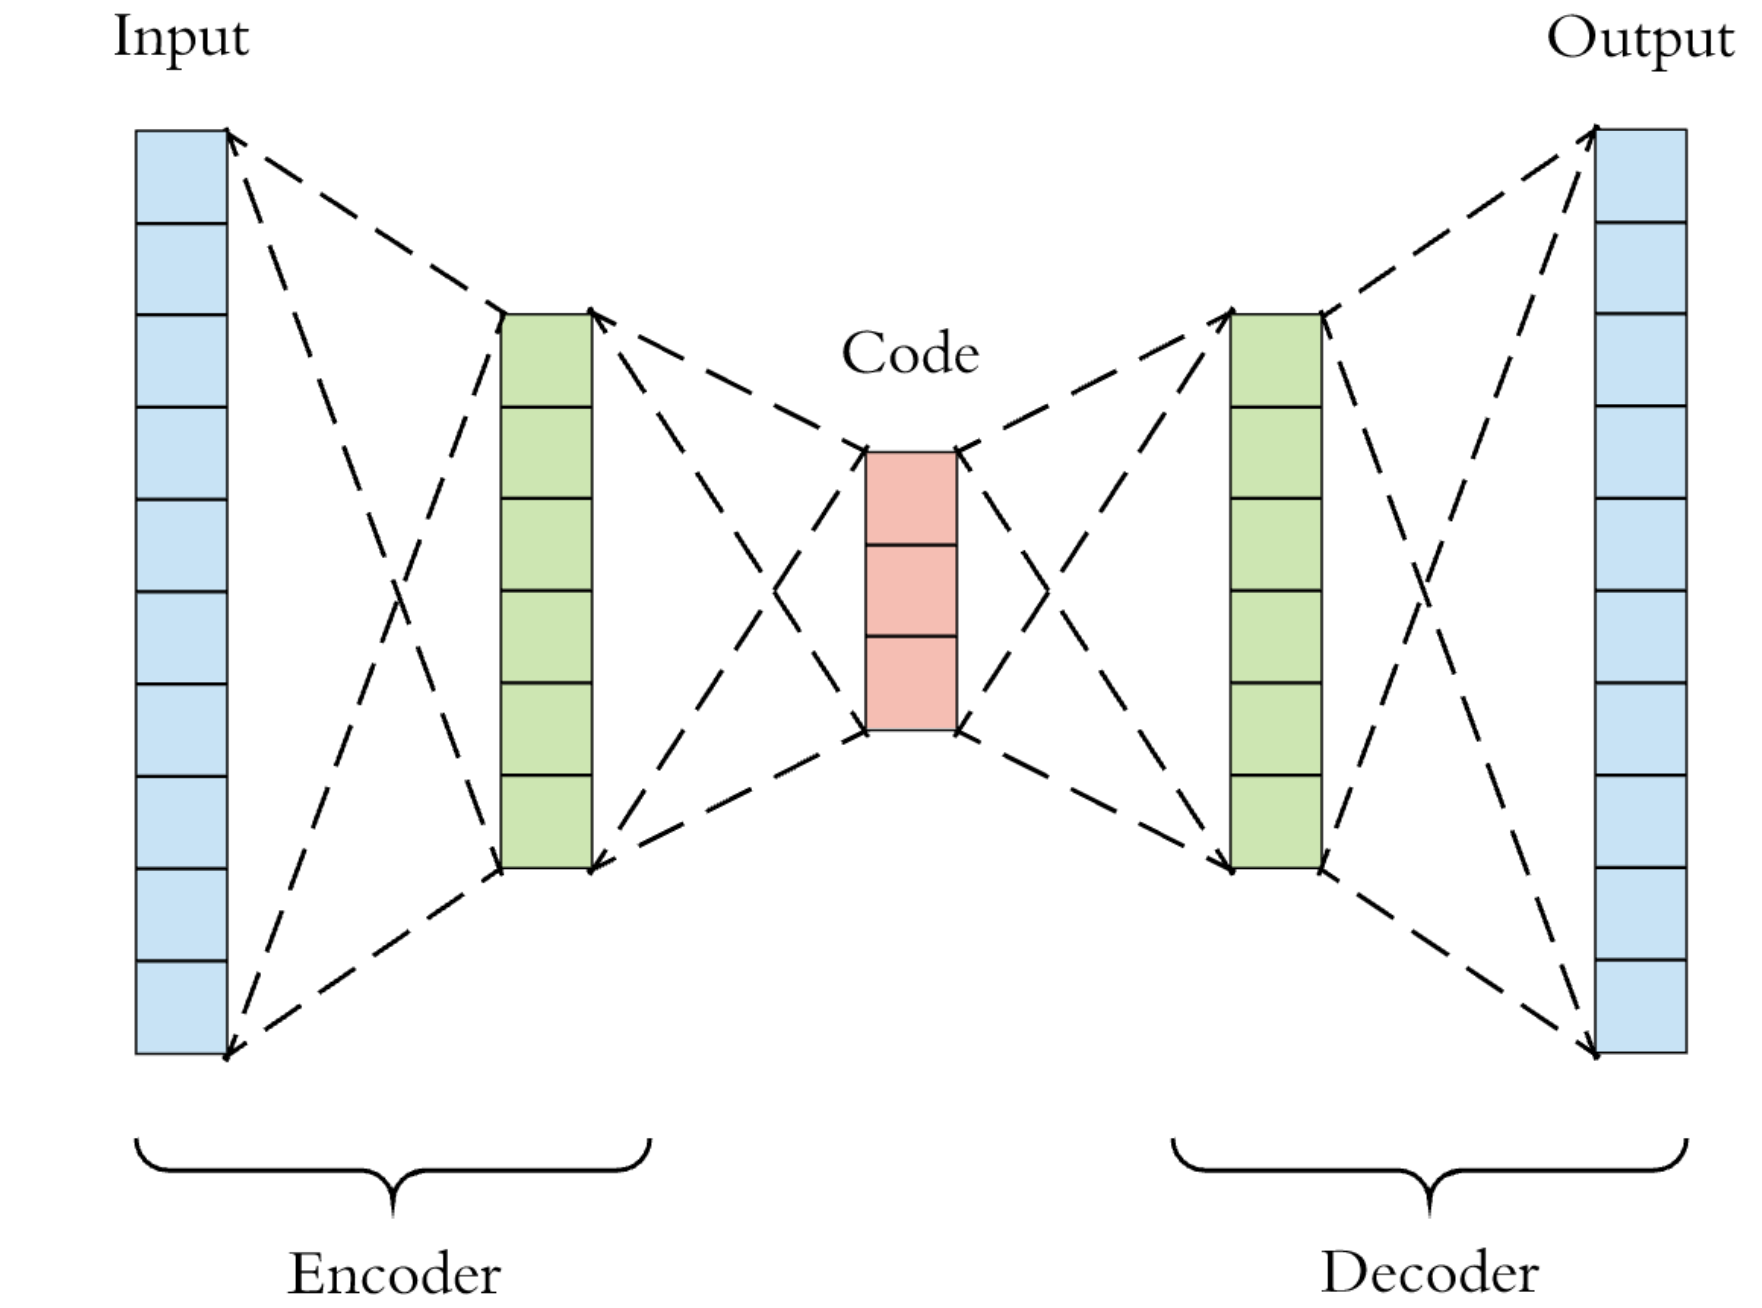
\includegraphics[width=.7\textwidth]{img/autoencoder}
  \caption{Esquema de un \textit{autoencoder}. Extraído de \parencite{arden_autoencoder_2017}.}
  \label{fig:autoencoder}
\end{figure}

La aplicación más directa de los \textit{autoencoders} es la reducción de
dimensionalidad para aprendizaje de características. Al forzar a la red a
codificar la entrada en un espacio de menos dimensión, la obligamos a abstraer
de ellas ciertas características que, además, nos permiten reconstruir la
imagen.

En el caso más simple donde solo existe una capa oculta, la fase de codificación
toma $\pmb x \in \mathbb{R}^p$ y devuelve $\pmb h \in \mathbb{R}^d$ con $d < p$ de la
forma
\[
\pmb h = \sigma (\pmb W \pmb x+\pmb b),
\]
donde $\sigma$ es una función de activación (sigmoide o ReLu), $\pmb W$ es una matriz
de pesos y $\pmb b$ es un vector de sesgo. Los pesos y el sesgo se suelen inicializar
de forma aleatoria y se van actualizando mediante \textit{backpropagation}.
Despues el codificador reconstruye $\pmb x'$ de la misma dimensión que $\pmb x$, haciendo
\[
\pmb x' = \sigma' (\pmb W' \pmb h + \pmb b'),
\]
donde $\sigma', \pmb W'$ y $\pmb b'$ no estan relacionados con sus equivalentes en el codificador. El \textit{autoencoder} busca entonces minimizar el error cuadrático, normalmente
referido como pérdida:
\[
\mathcal{L}(\pmb x, \pmb x') = \|\pmb x-\pmb x'\|^2 = \|\pmb x - \sigma'(\pmb W'(\sigma(\pmb W \pmb x + \pmb b))+ \pmb b')\|^2\,.
\]

\subsection{Redes neuronales recurrentes}%
\label{sub:redes_neuronales_recurrentes}

Las redes neuronales recurrentes, o RNN de forma abreviada, son una de las variantes de redes más importantes utilizadas en procesamiento de lenguaje natural.

En general, las redes neuronales convencionales procesan una entrada a través de un conjunto de capas y producen una salida, asumiendo que dos entradas consecutivas son independientes. Sin embargo, en escenarios de la vida real esto no siempre es cierto, siendo un ejemplo muy claro el intentar predecir la siguiente palabra de una oración, donde es primordial conocer el conjunto de palabras anteriores.

Las RNN intentan solucionar este problema realizando el mismo trabajo para cada elemento de una secuencia, dependiendo la salida de los cálculos previos. Es decir, se produce un fenómeno de \textit{retroalimentación} mediante el cual las capas de la red obtienen información de capas posteriores, y el flujo de infomación ya no es unidireccional. Esta diferencia es clave con respecto a las redes \textit{feed-forward}.

En teoría las redes recurrentes pueden usar información de secuencias de longitud arbitraria, pero en la práctica están limitadas a coger información de unos pocos pasos anteriores. Este problema se soluciona mediante el uso de redes de arquitectura \textit{long short-term memory}, que estan basadas en las RNN. En la Figura \ref{fig:rnn} mostramos un ejemplo de la estructura de una RNN.

\begin{figure}[h]
    \centering
    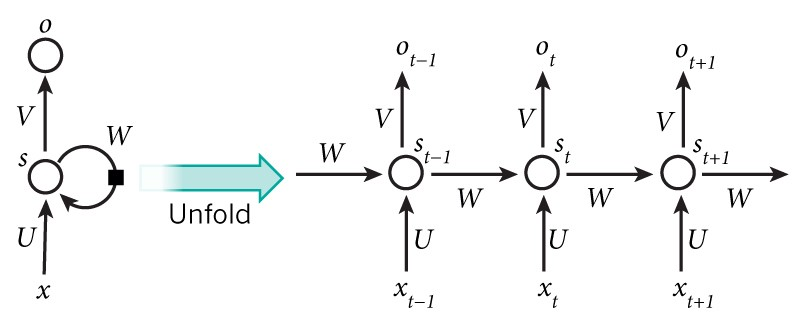
\includegraphics[width=0.7\linewidth]{img/rnn.jpeg}
    \caption{Ejemplo de red neuronal recurrente desenrrollada. Extraída de \parencite{nigam_understanding_2018}.}%
    \label{fig:rnn}
\end{figure}

\section{Ejemplos de aplicación de redes neuronales}
\label{sec:ejemplos}

\subsection{Codificación de imágenes en MNIST}

Vamos a ver un ejemplo donde entrenamos un \textit{autoencoder} sobre la base la base de datos MNIST \parencite{lecun_1998_gradient} para
codificar imágenes de números en un vector de valores reales. Esta base de datos contiene $70.000$ ejemplos de dígitos del 0 al 9 escritos a mano.

Utilizamos una red de 5 capas: dos capas para el codificador, una capa intermedia para el código y dos capas para el decodificador. Leeremos imágenes de tamaño 28x28 en escala de grises, que representaremos por un vector de píxeles con un valor entre 0 y 255. Cada neurona simulará un píxel, luego la primera capa tendrá $28 \times 28=784$ neuronas. Decidimos que la siguiente capa tendrá 128 neuronas y el código final, 4 neuronas. Luego subimos el tamaño nuevamente a 128 y finalmente a 784 neuronas, que será la imagen reconstruida. En la Figura \ref{fig:autoencoder_ex1}} podemos ver un ejemplo del resultado obtenido tras entrenar y evaluar la red.

\begin{figure}[h]
  \centering
  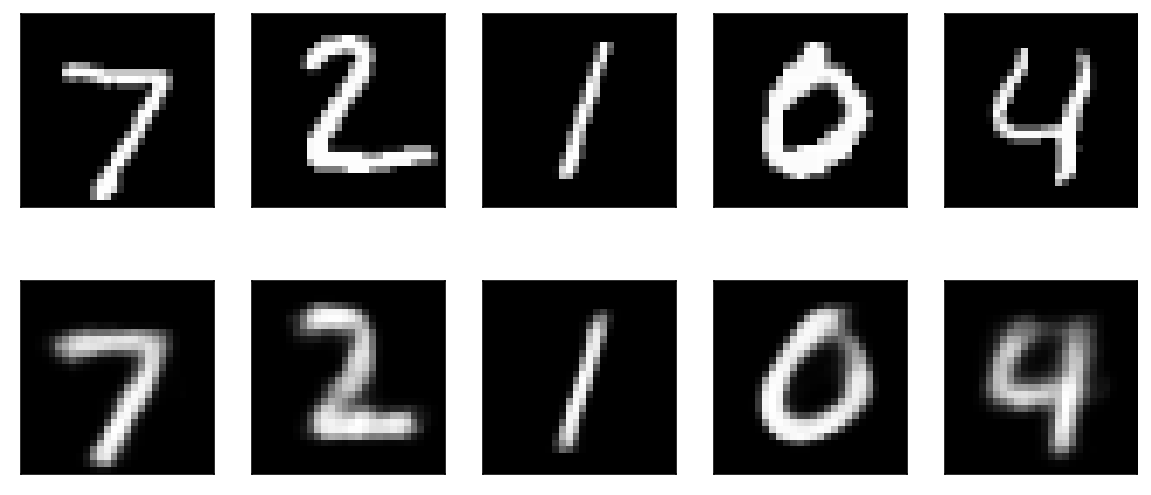
\includegraphics[width=.7\textwidth]{img/autoencoder_ex1}
  \caption{Ejemplo de ejecución del \textit{autoencoder} construido.}
  \label{fig:autoencoder_ex1}
\end{figure}

Si inspeccionamos el código de la primera imagen observamos que efectivamente es un vector de 4 números reales, que podríamos utilizar en alguna aplicación posterior para identificarla de forma unívoca:
$$\{13.325841  , 16.394411  , 13.2127905 ,  0.90243316\}.$$

También podemos utilizar el \textit{autoencoder} para eliminar ruido de
imágenes. Si entrenamos la red para que dada una entrada de imágenes con ruido, las codifique e iguale la salida a las imágenes sin ruido, podemos utilizar la red para hacer lo mismo con futuras imágenes. Un ejemplo de esta técnica se puede observar en la Figura \ref{fig:autoencoder_ex2}.

\begin{figure}[h]
  \centering
  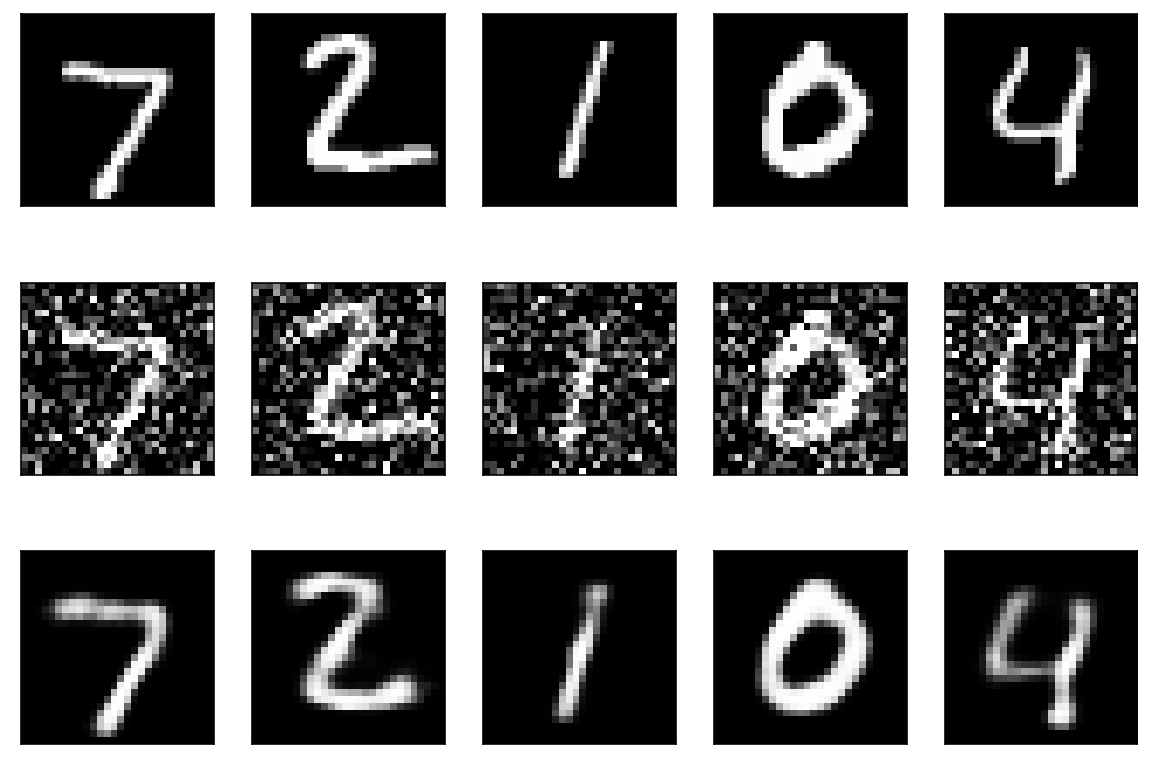
\includegraphics[width=.7\textwidth]{img/autoencoder_ex2}
  \caption{Ejemplo de ejecución del \textit{autoencoder} para eliminar ruido.}
  \label{fig:autoencoder_ex2}
\end{figure}

\subsection{Clasificación de imágenes en CIFAR-10}

El conjunto de datos CIFAR-10 \parencite{rizhevsky_learning_2009} consta de $60.000$ imágenes en color de 32x32 píxeles divididas en 10 clases, con $6.000$ imágenes por clase. A su vez se realiza una división en en $50.000$ imágenes para el conjunto de entrenamiento y $10.000$ imágenes en para el conjunto de test.

Las clases en las que se pueden clasificar las imágenes, como vemos en la Figura \ref{fig:cifar10}, son las siguientes: aviones, coches, pájaros, gatos, ciervos, perros, ranas, caballos, barcos y camiones. Las clases son completamente exclusivas, es decir, no hay parecidos entre clases similares, por ejemplo ningún coche se podrá confundir con un camión.

\begin{figure}[h]
  \centering
  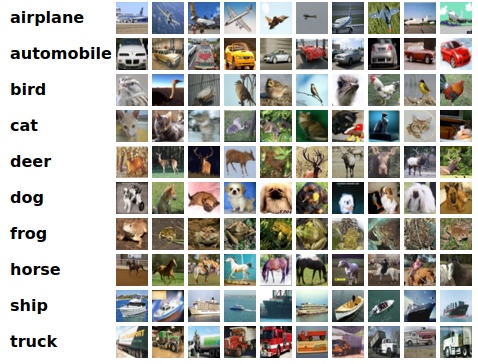
\includegraphics[width=.7\textwidth]{img/cifar10}
  \caption{Clases del conjunto de datos CIFAR10.}
  \label{fig:cifar10}
\end{figure}

FALTA EXPLICAR EL MODELO

\begin{figure}[h]
  \centering
  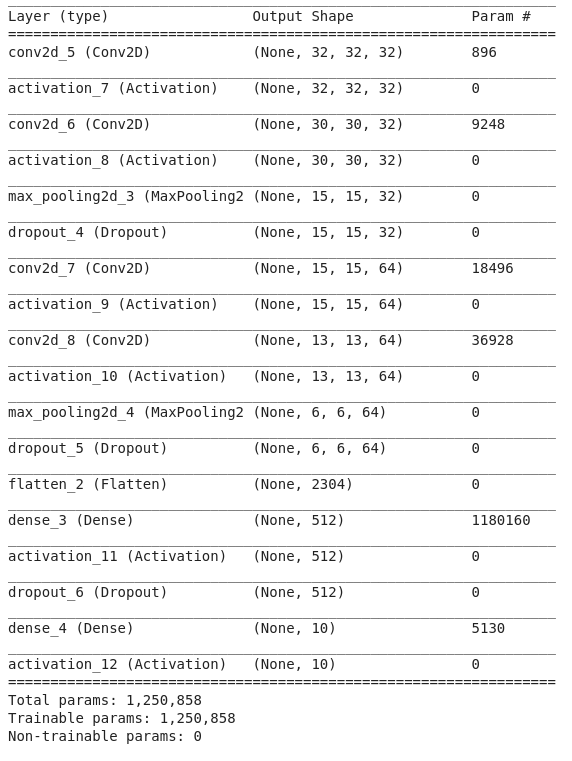
\includegraphics[width=.7\textwidth]{img/model}
  \caption{Capas de la red convolucional construida.}
  \label{fig:model}
\end{figure}

%%TODO: citar modelos de encoder y red usados. ¿Poner código github?

%-------------------------------------------------------------------------------
%	BIBLIOGRAFÍA
%-------------------------------------------------------------------------------

\newpage
\printbibliography

\end{document}
